\subsection{GAN avec spectrogramme}


\subsubsection{Modèle de base}
Le modèle de générateur initial était conçu avec une structure très simplifiée, comprenant principalement une couche de convolution unique après une transformation linéaire. La configuration de ce modèle se décompose comme suit :

\begin{itemize}
    \item Une couche entièrement connectée qui projette le vecteur latent \( z \) dans un espace de dimensions adaptées pour la mise en forme en image.
    \item Une redimensionnement de la sortie de la couche linéaire pour correspondre à un format d'image tri-dimensionnel, préparant les données pour la convolution.
    \item Une seule couche de convolution pour transformer l'image traitée par la couche précédente, utilisant une fonction d'activation tanh pour normaliser les sorties dans l'intervalle \([-1,1]\).
\end{itemize}

Ce modèle simplifié présente plusieurs limitations :

\paragraph{Manque de profondeur}
Avec une seule couche de convolution, le réseau est limité dans sa capacité à extraire et à recomposer des caractéristiques complexes des données d'entrée

\paragraph{Problèmes de généralisation}
Le modèle souffre également de sous-apprentissage, car les valeurs des pertes du discriminateur et du générateur ne convergent pas. La perte du discriminateur reste très basse, généralement entre 0 et 1, tandis que celle du générateur fluctue considérablement, reflétant la performance variable du réseau de neurones.

\paragraph{Résolution et détails}
Il est également difficile pour le modèle de capturer les détails ; plusieurs couches supplémentaires sont nécessaires pour qu'il puisse générer des images avec une finesse accrue.

\begin{figure}[ht]
    \centering
    \begin{subfigure}[b]{0.45\textwidth}
        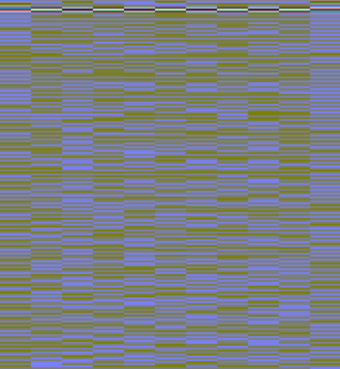
\includegraphics[width=\textwidth]{logos/real_sample.png}
        \caption{Exemple d'image d'entrainement}
        \label{fig:image1}
    \end{subfigure}
    \hfill % Espacement entre les images
    \begin{subfigure}[b]{0.45\textwidth}
        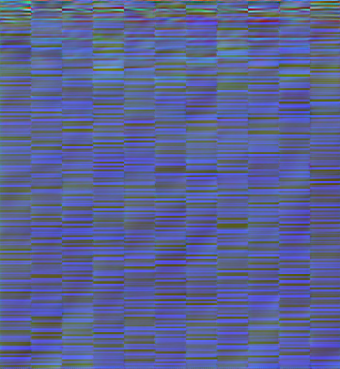
\includegraphics[width=\textwidth]{logos/generated_samples1.png}
        \caption{Première image générée avec le modèle de base au bout d'une heure d'entraînement.}
        \label{fig:image2}
    \end{subfigure}
    \caption{Images côte à côte}
    \label{fig:images_cote_a_cote}
\end{figure}


\subsubsection{Modèle amélioré}
La deuxième modification majeure concernait l'introduction de couches de convolution supplémentaires dans l'architecture du générateur. Cette modification visait à améliorer la capacité du modèle à capturer et à reproduire des détails plus fins dans les images générées. Les couches ajoutées ont permis une hiérarchisation plus complexe des traits caractéristiques, ce qui a entraîné une augmentation notable de la qualité visuelle des spectrogrammes produits.

\begin{figure}[H]
    \centering
    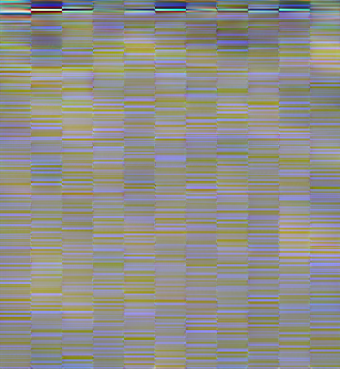
\includegraphics[width=0.8\textwidth]{logos/generated_samples2.png}
    \caption{Impact de la modification sur la qualité des images générées}
    \label{fig:mod2}
\end{figure}

Cette amélioration est visible dans les images générées, où les textures et les gradients sont plus naturels et mieux définis par rapport au modèle initial. Cette approche a également contribué à une convergence plus stable des fonctions de perte pendant l'entraînement.


Illustration des changements de performance ou de qualité des résultats.
\begin{figure}[H]
    \centering
    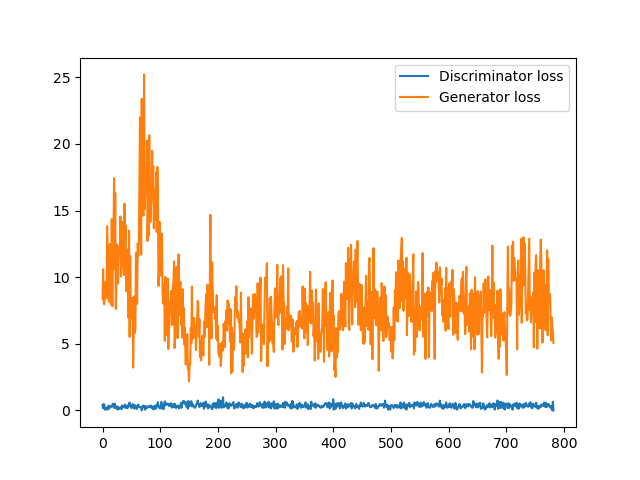
\includegraphics[width=0.4\textwidth]{logos/loss.png}
    \caption{Impact de la Modification 2}
    \label{fig:mod2}
\end{figure}

\subsubsection{Prochaines idées et pistes}
Pour poursuivre l'amélioration de notre modèle GAN pour la génération de spectrogrammes, plusieurs pistes peuvent être envisagées :

\begin{itemize}
    \item \textbf{Augmentation des données :} L'introduction de techniques d'augmentation de données plus variées pourrait aider le modèle à mieux généraliser et à produire des résultats de meilleure qualité sur des données non vues lors de l'entraînement.
    \item \textbf{Optimisation des hyperparamètres :} Un tuning plus fin des hyperparamètres, notamment les taux d'apprentissage et le nombre de couches, pourrait potentiellement améliorer la stabilité et l'efficacité de l'apprentissage.
    \item \textbf{Exploration d'architectures avancées :} L'expérimentation avec des architectures de réseau plus complexes, telles que les GANs conditionnels ou les réseaux adversariaux auto-encodeurs, pourrait ouvrir la voie à des améliorations significatives de la qualité des images.
\end{itemize}

Ces initiatives devraient être guidées par des validations expérimentales continues et des comparaisons rigoureuses pour évaluer leur efficacité réelle dans la production de spectrogrammes réalistes et utiles.
